\documentclass{article}
\usepackage[spanish]{babel}
\usepackage[margin = 2cm]{geometry}
\usepackage{amsmath, amssymb}
\usepackage{caption}
\usepackage{graphicx}
\DeclareCaptionType{equ}[][]
\title{Calculo de Estimadores Usando Metodos Numericos}
\author{Rudy Miranda}
\date{\today}
\begin{document}
    \maketitle
    
    \section{Introduccion}

    \section{Ejemplo Distribucion Exponencial}

    \subsection{Estimador Maximo Verosimil}
    \begin{align}
        L(\lambda) &= \Pi_{i=1}^{n} \lambda e^{-\lambda x_{i}} \\
                   &= \lambda^{n} e^{-\lambda \sum_{i}^{n} x_{i}}
    \end{align}
    
    Aplicamos $\log$ a ambos lados

    \begin{align}
        log(L(\lambda )) &= log\left(\lambda^{n} e^{-\lambda \sum_{i}^{n} x_{i}}\right) \\
                         &= nlog(\lambda) -\lambda \sum x_{i}
    \end{align}
    
    y esta es nuestra funcion a maximizar. Notar que solo depende de $\lambda$, ya que $n$ es el tamano de la muestra y $\sum x_{i}$ es la suma de todas las observaciones.

    Usando herramientas de calculo,

    \begin{equation}
        \frac{d log L(\lambda)}{d\lambda} = \frac{n}{\lambda} - \sum x_{i} = 0 \quad \Rightarrow \quad \hat{\lambda} = \frac{n}{\sum x_{i}} = \left(\frac{\sum x_{i}}{n} \right )^{-1} = \bar{x}^{-1}
    \end{equation}

    procedemos a evaluar la segunda derivada en $\bar{x}^{-1}$

    \begin{equation}
        \frac{d^{2} L(\lambda)}{d \lambda^{2}} = -\frac{n}{\lambda^{2}} \quad \Rightarrow \quad \frac{d^{2} L(\lambda)}{d \lambda^{2}} \Big|_{\lambda = \bar{x}^{-1}} = -\frac{n}{(\bar{x}^{-1})^{2}} < 0
    \end{equation}

    De esta forma encontramos el estimador de forma analitica.

    \subsubsection{Usando \textit{R}}
    Una forma sencilla de maximizar funciones en \textit{R} es con el comando \verb|optimize|.
    
    \subsubsection*{Input:}
    \begin{verbatim}
n <- 100
muestra <- rexp(n, rate = 2)
sum_m <- sum(muestra) #53.71737
f <- function(lambda) {
    n * log(lambda) - lambda * sum_m
}
optimize(f, interval = c(1, 3), maximum = TRUE)
1 / mean(muestra)\end{verbatim}
    
    \subsubsection*{Output:}
    \begin{verbatim}
> optimize(f, interval = c(1, 3), maximum = TRUE)
$maximum
[1] 1.861609
> 1/mean(muestra)
[1] 1.861595\end{verbatim}
    
    \subsubsection{Usando \textit{C}}
    En \textit{C} lo podemos hacer usando Newton-Rhapson.

    \subsubsection*{Input:}
    \begin{verbatim}
#include <stdio.h>
#include <math.h>
int main(){
    int reps = 100; // Numero Maximo de
                    // Iteraciones
    float temp, aux = 1, n = 100, sum_x = 53.71737, epsilon = 0.05;
    for(int i = 0; i < reps; i++){
        temp = aux;
        aux = aux - (n/aux - sum_x)/(-n/pow(aux, 2));
        if(fabs(aux - temp) < epsilon)
            break;
    }
    printf("Raiz por Newton Rhapson: %f\n", aux);
    return 0;
}\end{verbatim}

    \subsubsection*{Output:}
    \begin{verbatim}
Raiz por Newton Rhapson: 1.861587\end{verbatim}
    \subsubsection{Usando \textit{MATLAB}}
    Tambien una herramienta util seria \textit{MATLAB} (o \textit{Octave}), ya que en este las funciones pueden recibir como argumentos otras funciones, lo cual sera muy util en el caso multimensional cuando necesitemos usar la matriz jacobiana en el metodo de Newton.
    
    \section{Ejercicio Libro seccion 5.5.2}
    En el ejemplo del libro se pide ajustar una funcion de densidad a un histograma. La funcion de densidad pedida es la de la distribucion gamma, donde lo primero a hacer es estimar los parametros.

    Para estimar los parametros hay dos metodos que se aprenden en Inferencia I, los cuales son: Metodo de los Momentos y Metodo de Maxima Verosimilud.
    \begin{equ}[!ht]
        \begin{equation*}
            f(x; a, b) = \frac{b^a}{\Gamma(a)} x^{a-1} e^{-bx},\quad a > 0,\hspace{0.1cm} b > 0,\hspace{0.1cm} x \in (0, \infty)
        \end{equation*}
        \caption*{Funcion de Densidad D. Gamma}
    \end{equ}

    \subsection{Metodo de los Momentos}
    Este metodo consiste en igualar momentos poblacionales con momentos muestrales tantas veces como parametros hayan.

    \begin{align}
        \mathrm{E}(X) &= \int_{0}^{\infty} x \cdot \frac{b^a}{\Gamma(a)} x^{a-1} e^{-bx} \, \mathrm{d}x \\
                      &= \int_{0}^{\infty} \frac{b^a}{\Gamma(a)} x^{(a+1)-1} e^{-bx} \, \mathrm{d}x \\
                      &= \int_{0}^{\infty} \frac{1}{b} \cdot \frac{b^{a+1}}{\Gamma(a)} x^{(a+1)-1} e^{-bx} \mathrm{d}x \\
                      &= \int_{0}^{\infty} \frac{a}{b} \cdot \frac{b^{a+1}}{\Gamma(a+1)} x^{(a+1)-1} e^{-bx} \, \mathrm{d}x \\
                      &= \frac{a}{b} \int_{0}^{\infty} \mathrm{Gam}(x; a+1, b) \mathrm{d}x \\
                      &= \frac{a}{b}
    \end{align}

    Tenemos que la media es $\frac{a}{b}$. En cuanto a la varianza, esta la calcularemos en funcion del primer y segundo momento

    \begin{align}
        \mathrm{E}(X^2) &= \int_{0}^{\infty} x^2 \cdot \frac{b^a}{\Gamma(a)} x^{a-1} e^{-bx} \, \mathrm{d}x \\
                        &= \int_{0}^{\infty} \frac{b^a}{\Gamma(a)} x^{(a+2)-1} e^{-bx} \, \mathrm{d}x \\
                        &= \int_{0}^{\infty} \frac{1}{b^2} \cdot \frac{b^{a+2}}{\Gamma(a)} x^{(a+2)-1} e^{-bx} \, \mathrm{d}x \; . \\
                        &= \int_{0}^{\infty} \frac{a \, (a+1)}{b^2} \cdot \frac{b^{a+2}}{\Gamma(a+2)} x^{(a+2)-1} e^{-bx} \, \mathrm{d}x \\
                        &= \frac{a \, (a+1)}{b^2} \int_{0}^{\infty} \mathrm{Gam}(x; a+2, b) \, \mathrm{d}x \\
                        &= \frac{a^2+a}{b^2}
    \end{align}

    Entonces, 

    \begin{align}
    \mathrm{Var}(X) &= \frac{a^2+a}{b^2} - \left( \frac{a}{b} \right)^2 \\
                    &= \frac{a}{b^2} \; .
    \end{align}

    Procedemos a generar un sistema de ecuaciones:
    \begin{align}
        \bar{x} &= \frac{a}{b} \\
        s^2 &= \frac{a}{b^2}
    \end{align}

    de $(22)$ tenemos que 
    \begin{align}
        a = s^2 b^2 \Rightarrow \bar{x} &= \frac{s^2 b^2}{b}\\
                                        &= b s^2 \\
        \hat{b}_{mm} &= \frac{\bar{x}}{s^2}
    \end{align}

    Sustituyendo $b$ en $(22)$

    \begin{align}
        s^2 &= \frac{a}{\left(\frac{\bar{x}}{s^2} \right)^2} \\
            &= \frac{a (s^2)^2}{\bar{x}^2} \Rightarrow \hat{a}_{mm} = \frac{\bar{x}^2}{s^2}
    \end{align}

    De esta forma encontramos la solucion analitica presente en la pagina 114 del libro.
    \subsection{Metodo de Maxima Verosimilud}
    \begin{align}
        L(a, b) &= \Pi_{i=1}^{n} \frac{b^a}{\Gamma(a)} x_{i}^{a-1} e^{-bx_i}\\
                &= \left(\frac{b^a}{\Gamma (a)}\right)^n e^{-b\sum_{i=1}^{n}x_i} \Pi_{i=1}^n x_i^{a-1}
    \end{align}
    Aplicamos $\log$
    \begin{align}
        \log L(a,b) &= n\log\left(\frac{b^a}{\Gamma (a)}\right ) -b\sum_{i=1}^{n}x_i + \sum_{i}^{n} \log x_i^{a-1} \\
                    &= na\log b - n\log\Gamma(a) -b\sum_{i=1}^{n}x_i + (a-1)\sum_{i}^{n} \log x_i
    \end{align}

    Esta funcion ya es optimizable en \textit{R} con las funciones \verb|optim| y \verb|nlminb|, pero veremos que podemos dejar la funcion solo en termino de $a$.

    \begin{equation}
        \frac{\partial \log L(a, b)}{\partial b} = \frac{na}{b}-\sum_{i=1}^nx_i \Rightarrow \hat{b} = \frac{a}{\bar{x}} 
    \end{equation}

    Sustituimos en $(31)$,

    \begin{equation}
        log L(a) = na\log \frac{a}{\bar{x}} - n\log\Gamma(a) - \frac{a}{\bar{x}}\sum_{i=1}^{n}x_i + (a-1)\sum_{i}^{n} \log x_i
    \end{equation}

    \subsubsection{Resolviendo con Newton-Rhapson}
    Necesitamos encontrar las primeras dos derivadas de la funcion de verosimilitud.

    \begin{equation}
        \frac{\partial log L(a)}{\partial a} = n (1 + log\frac{a}{\bar{x}}) -n \frac{1}{\Gamma (a)} \Gamma'(a) - n + \sum_{i=1}^{n} log x_i
    \end{equation}

    \begin{equation}
        \frac{\partial^2 logL(a)}{\partial a^2}= \frac{n}{a} - n\frac{\Gamma ''(a)\Gamma (a) - (\Gamma ' (a))^2}{(\Gamma (a))^2}
    \end{equation}
    \section{Ajuste de Curva}
    Generamos una muestra y graficamos su histograma
    \begin{verbatim}
n <- 500
x <- rgamma(n, shape = 2, rate = 3)
hist(x, breaks = 15, freq = FALSE, col = "cyan")\end{verbatim}
    \newpage
    \begin{figure}[ht]
        \centering
        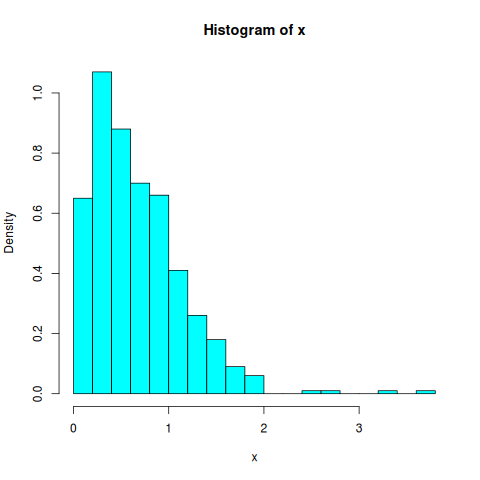
\includegraphics[width = 0.35\textwidth]{example2.png}
    \end{figure}

    \subsection{Curva con Estimadores por Metodo de los Momentos}
    \subsubsection{Input:}
    \begin{verbatim}
a <- mean(x)^2 / var(x)
b <- mean(x) / var(x)
c1gamma <- function(y) dgamma(y, a, b)
hist(x, breaks = 15, freq = FALSE, col = "cyan")
curve(c1gamma, lwd = 2,  add = TRUE)\end{verbatim}
    \subsubsection{Output:}
    \begin{verbatim}
> a
[1] 2.005734
> b
[1] 2.979978\end{verbatim}
    
    \begin{figure}[ht]
        \centering
        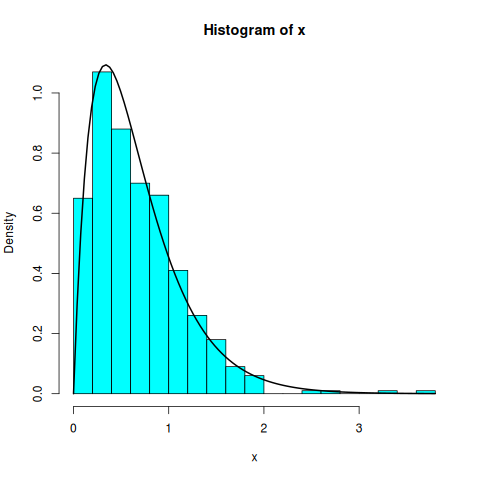
\includegraphics[width = 0.4\textwidth]{mm.png}
    \end{figure}

    \subsection{Curva con Estimadores por Metodo de Maxima Verosimilud}
    \subsubsection{Maximizacion con funcion \textit{optimize}}
    \subsubsection*{Input:}
    \begin{verbatim}
loglh <- function(a) {
    n * a * log(a / xbar) - n * log(gamma(a))- a * n + (a - 1) * sum(log(x))
}
optimize(loglh, interval = c(1, 3), maximum = TRUE)
a <- 1.882421
b <- a / mean(x)
c3gamma <- function(y) dgamma(y, a, b)
hist(x, breaks = 15, freq = FALSE, col = "cyan")
curve(c3gamma, lwd = 2,  add = TRUE)\end{verbatim}
    \subsubsection*{Output:}
    \begin{verbatim}
> optimize(loglh, interval = c(1, 3), maximum = TRUE)
$maximum
[1] 1.882421

$objective
[1] -252.6241\end{verbatim}
    \begin{figure}[ht]
    \centering
        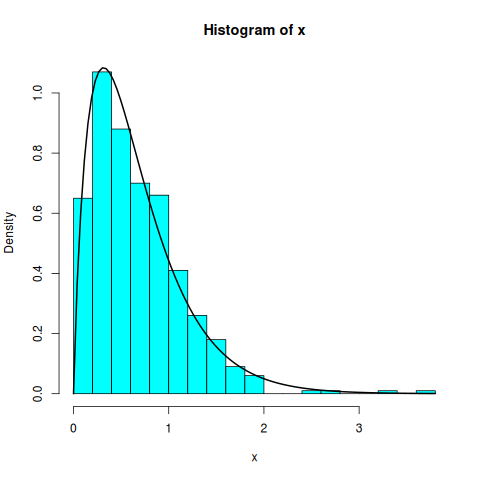
\includegraphics[width = 0.4\textwidth]{optim.png}
    \end{figure}
    \subsubsection{Maximizacion por Newton-Rhapson}
    \subsubsection*{Input:}
    \begin{verbatim}
xbar <- mean(x)
epsilon <- 0.0001 # criterio de detencion
f <- function(a) {
    n * (1 + log(a) - log(xbar)) - n * digamma(a) - n + sum(log(x))
}
df <- function(a) { # derivada de f
    n / a - n * trigamma(a)
}
aux <- 1.5 # aproximacion inicial
for (i in 1:100){
    temp <- aux
    aux <- aux - f(aux) / df(aux)
    if (abs(aux - temp) < epsilon)
        break
}
c2gamma <- function(y) dgamma(y, aux, aux / mean(x))
hist(x, breaks = 15, freq = FALSE, col = "cyan")
curve(c2gamma, lwd = 2,  add = TRUE)\end{verbatim}
    \subsubsection*{Output:}
    \begin{verbatim}
> aux
[1] 2.169999
> aux / mean(x)
[1] 3.224033\end{verbatim}
    \begin{figure}[ht]
        \centering
        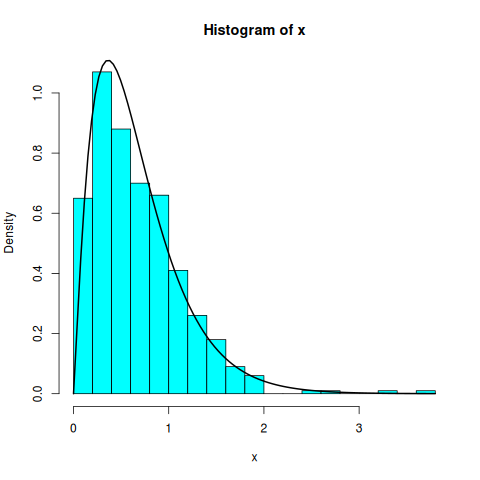
\includegraphics[width = 0.4\textwidth]{mmv.png}
    \end{figure}
\end{document}
